\section{Architecture}
In this section we have used design by intuition to create the overall architecture of how the system will work. Our argument for doing so is because we lack domain knowledge with using a tool as the one we are about to create. We will only gain this knowledge after we have spent time working on our first implementations of the DSL. Hopefully the development process will guide us to a more defined and fit for purpose architecture.

\subsection{Logical View}
Most of the objectives listed in the Objectives section(p.\pageref{sec:objectives}) are concerned with the ability of implementing the Diffie-Hellman-Merkle key exchange protocol. For our architecture we want to be more general in which protocol we implement. We will focus on creating a foundation for implementing an arbitrary protocol. Afterwards we will see if we need to add or change features to be able to implement a more complex protocol.

\begin{figure}[h]
	\centering
	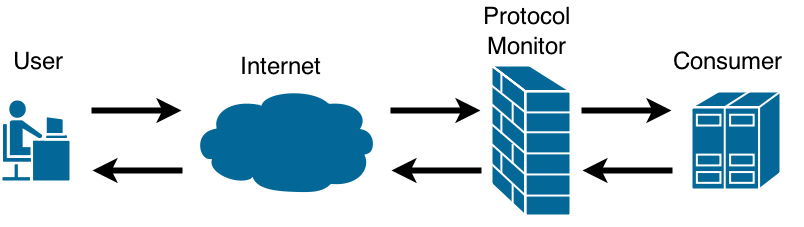
\includegraphics[scale=0.45]{images/architecture/ArchitectureFigure1.png} 
	\caption{Logical View of the architecture}
	\label{fig:ArchitectureFigure1}
\end{figure}
Figure \ref{fig:ArchitectureFigure1} shows the overall design for our concept. 
\\
Users must connect through the internet to reach the Consumer. A Consumer is the entity that ''consumes`` the messages\footnote{A message is used to represent a package being sent from one client to the other} that get sent from the Protocol Monitor (PM). A message that goes through the PM must be the expected outcome of the protocol.
\\\\
The PM is drawn as a firewall because it will act in the same way as a firewall does: it has rules that govern what messages are allowed to pass through. The rules contained within the PM will be defined by our DSL.
\\\\
If a message is attempted to be sent or received and it breaks the protocol, the connection is to be terminated. Attempting to repair the connection would in most cases lead to the same error being thrown. Instant termination of the connection would however make both parties aware that the protocol has been broken. There should however be some form of construct that allows for a protocol to branch. This could be added to facilitate the use of multiple versions of a protocol in production.
\\\\
At a later stage we will need to decide at what level the PM ensures that a protocol is obeyed. For simpler protocols we should be able to guaranty full protocol compliance. This becomes much harder to achieve in the case of when a consumer is expecting to receive an encrypted value and that value must have certain properties. For the PM to be able to handle these types of events, it must have the means to decrypt the message.

\subsection{Protocol Monitor}
In order for the architecture to function as we have described, the PM requires certain features. First, it must be able to know if a message received/sent is what the protocol expects. For this to happen the PM must know the state the protocol is in. This state must contain the means of verifying if a new message is expected. The second requirement is that it must be able to act appropriately for the messages received. This includes passing messages along to the users/consumers and also being able to terminate a connection.
\subsubsection{Protocol state}
The task of the PM is to forward and validate messages it receives. For it to validate these messages, it must also contain a state. This state is the state that the defined protocol is in.
\\
Defining the state will be the task of the DSL. Defining such a protocol capable of containing such a fluctuating state needs to be as effortless as possible. The syntax should also be concise so that reasoning about how the protocol operates is obvious.

\subsection{Consumer and Client}
With our definition of what responsibilities the PM has, we can safely assume that all messages successfully sent and received by the consumer and client are valid. In this sense valid means that the message contains a accepted value and is in the correct order.
\subsubsection{Tasks}
The consumer and client must be programmed in such a way that they have handlers that can deal with the messages sent by the other party. They types of messages they receive can be derived directly from the protocol specification. 


\subsection{Mapping}
The task for the Protocol Monitor, Consumer and, optionally, the Client can be all implemented as actors as shown in figure \ref{fig:ArchitectureMapping}. The ``Client'' does not need to be implemented as an actor. Its only requirement is that it must obey the protocol. The Client side could for example be someone using telnet to communicate with the server.
\\
This solution will allow the ``Consumer'' to create additional actors in a hierarchy beneath itself. This would allow for more concurrency and distribute workload and state throughout a system. 
\begin{figure}[h]
	\centering
	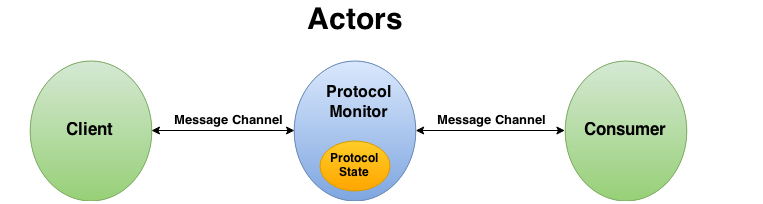
\includegraphics[scale=0.45]{images/architecture/ArchitectureMapping.png} 
	\caption{Representation of our Actors}
	\label{fig:ArchitectureMapping}
\end{figure}

The next part is to be able to define a protocol, the protocol state that the PM will use.






















